\documentclass[letterpaper]{article}
\usepackage[submission]{aaai2027}
\usepackage[hyphens]{url}
\usepackage{graphicx}
\urlstyle{rm}
\def\UrlFont{\rm}
\usepackage{natbib}
\usepackage{caption}
\usepackage{booktabs}
\frenchspacing
\pdfinfo{/TemplateVersion (2027.1)}
\setcounter{secnumdepth}{0}
\title{Which Dose Predictor Fits This Cohort?\\An Auditable Agent Design for Radiotherapy Model Selection}
\author{}
\affiliations{}
\begin{document}
\maketitle

\begin{abstract}
Radiotherapy dose prediction requires accurate estimates of both target coverage and dose to adjacent organs. The anatomical structures available to train and evaluate a predictor vary across patients, even within a single treatment site. We propose a tool-using agent for cohort-specific model selection. It would use measurements of target geometry, contour availability and dose gradients to propose changes to a SearchedNet architecture and its training hyperparameters. A separate matched comparison would test whether excluding records with a documented quality concern improves prediction. To assess the choice of search space, we compared a fixed 3D U-Net with NAS-29, a previously searched configuration, on 100 held-out OpenKBP head-and-neck patients. NAS-29 reduced mean dose error from 2.654 to 2.555 Gy and pooled dose--volume histogram (DVH) error from 1.809 to 1.663 Gy. Target coverage estimates improved, whereas spinal cord near-maximum dose error increased. These results motivate evaluating SearchedNet configurations against both voxelwise and structure-specific endpoints. Implementation and evaluation of the selection agent remain future work.
\end{abstract}

\section{Introduction}
In head-and-neck radiotherapy, the dose prescribed to a target may need to fall sharply over a short distance to spare the spinal cord. A predictor can reproduce most of the dose field yet misestimate dose in the small volume of cord closest to the target. OpenKBP addresses these complementary aspects of prediction through a voxelwise dose score and a dose--volume histogram (DVH) score computed from target and organ endpoints \citep{openkbp}. For model selection, the implications are concrete: a reduction in mean voxel error warrants examining which structures account for the improvement and which remain poorly predicted.

Given a planning computed tomography (CT) image and contours of planning target volumes (PTVs) and organs at risk (OARs), we aim to predict the three-dimensional reference dose in gray (Gy). Converting such a prediction into a deliverable plan requires a further optimization step subject to machine constraints and planning objectives \citep{planning}. The proposed agent operates during model development. At inference, the selected network takes the contoured CT as input and produces a dose field.

U-Net provides a common encoder--decoder architecture for biomedical images \citep{unet}. In head-and-neck dose prediction, dense connections and dilated convolutions have also been incorporated into a 3D U-Net \citep{gronberg}. Training adjusts the weights of such a network, while the choice of receptive field, resolution changes and decoder operations is fixed in advance. The suitability of those choices may depend on target size, target--organ separation and how often an organ is contoured. We propose to treat each of these dependencies as a testable hypothesis by specifying a component substitution and an endpoint before training.

We use SearchedNet as the initial candidate family because its encoder and decoder operations can be varied within a common topology. We evaluate this choice by comparing one configuration from the LENAS search space, NAS-29 \citep{lenas}, with a fixed 3D U-Net under the same training protocol. Alongside cohort-level dose and DVH scores, we compare cumulative DVH curves to identify differences in target coverage and organ dose. The lower aggregate errors obtained with NAS-29 on this cohort motivate a second question: under a fixed search budget, do proposals informed by training-set measurements yield better predictors than sampling the same search space?

\section{Problem and Design Precedents}
For patient $i$, let $X_i$ contain CT intensities and target and organ masks on a common grid, $D_i$ be the reference dose in Gy, and $M_i$ the voxels in which dose can be deposited. A predictor $f_\theta(X_i)$ estimates a scalar at each voxel. We score its spatial accuracy for this patient by
\begin{equation}
 e_i=\frac{1}{|M_i|}\sum_{v\in M_i}
 \left|f_\theta(X_i)_v-D_{iv}\right|.
\end{equation}
The organ masks identify anatomical structures even where they overlap a dose gradient. A cumulative dose--volume histogram (DVH) gives the fraction of a structure receiving at least a given dose. Two fields can have similar DVHs while assigning dose to different voxels. Conversely, a small structure can contribute little to $e_i$ despite a large error at its high-dose end. We therefore keep both spatial and DVH errors in the selection record.

Prior work adapts different parts of an imaging pipeline to the data. In segmentation, nnU-Net uses dataset properties to configure preprocessing, network architecture and training \citep{nnunet}. In dose prediction, nnDoseNet adapts this approach to a continuous dose target and compares training configurations \citep{nndose}. DoseDiff incorporates anatomical geometry directly into the predictor through distance maps \citep{dosediff}. LENAS searches architectural blocks and uses ensembles and knowledge distillation to exploit variation among predictors \citep{lenas}. Our proposed contribution concerns the selection procedure: linking a measured cohort property to a specific change in data inclusion, architecture or training, and recording the trial that supports or contradicts that choice.

\subsection{Variation in Training Contours}
OpenKBP provides synthetic reference plans for head-and-neck cases. Prediction error therefore measures agreement with a benchmark planning protocol. The split comprises 200 training, 40 validation, and 100 test patients \citep{openkbp}. Table~\ref{tab:cohort} describes the training contours used here. We calculated each volume by multiplying its number of delineated voxels by the patient's voxel volume and converting to milliliters. All 200 cases contain a 70 Gy target, but its largest volume is over two orders of magnitude greater than its smallest. The esophagus contributes a contour in only 81 cases. A missing contour is therefore relevant both to the model input and to the number of patients who can support an esophageal endpoint. It gives no measurement of that patient's esophageal dose error.

\begin{table}[t]
\centering
\begin{tabular}{lrrr}
\toprule
Contour & Cases & Median (mL) & Range (mL)\\
\midrule
PTV70 & 200 & 291.15 & 9.02--1245.13\\
Brainstem & 182 & 25.42 & 4.87--47.54\\
Spinal cord & 188 & 25.58 & 5.34--57.04\\
Esophagus & 81 & 11.68 & 2.20--40.87\\
Larynx & 100 & 24.08 & 0.53--85.84\\
\bottomrule
\end{tabular}
\caption{Selected training contours. Volume summaries include only patients with the respective contour. Each patient contributes one observation per row.}
\label{tab:cohort}
\end{table}

The proposed profiling tool would extend these summaries in two directions. First, it would calculate the nearest distance in millimeters from each delineated OAR to the union of the PTVs and the fraction of that organ overlapping a target. Second, it would estimate the reference dose gradient in Gy/mm in a 3 mm inner band along the organ boundary, using the physical spacing along each axis. Recording the count of usable patients and voxels matters: a high percentile estimated in a thin boundary band can depend on only a few measurements. These are proposed inputs to search. The measured contour volumes alone do not establish that any operator performs better on small targets.

\section{A Proposed Agent for Model Development}
The proposed controller takes patient manifests, an output directory and a compute budget as inputs. Local tools handle images, measure cohort properties and execute training jobs. They return statistics, effective configurations, job identifiers and artifact locations. These records support three decisions: which cases are eligible for training, which architecture and hyperparameters to advance, and whether the selected predictor benefits from a more restrictive training manifest. The completed baseline experiments used the original training set and manually specified configurations.

\begin{table*}[t]
\centering
\begin{tabular}{lp{3.00in}ll}
\toprule
Position in cell & Allowed operations & Encoder in NAS-29 & Decoder in NAS-29\\
\midrule
Main path, first & Identity, standard convolution, depthwise separable convolution, dilated convolution, SE channel weighting & Identity & Depthwise separable\\
Main path, second & Same five choices, selected independently & Dilated & Depthwise separable\\
Local branch & Identity or zero operation & Zero & Zero\\
Encoder exit & Average pooling, max pooling, or stride-2 convolution (standard, depthwise separable, dilated, or SE) & Depthwise separable & ---\\
Decoder exit & Transposed convolution (standard, depthwise separable, dilated, or SE), or convolution followed by trilinear interpolation & --- & Trilinear variant\\
\bottomrule
\end{tabular}
\caption{Complete component choices in the implemented SearchedNet space. SE denotes squeeze-and-excitation. Operator names describe the weight operation within the implementation's activation and normalization wrapper. The two rightmost columns specify all eight choices in the completed NAS-29 experiment.}
\label{tab:ops}
\end{table*}

\subsection{Screening the training records}
The data preparation tool would verify that reference doses are readable and finite, that CT, dose and masks share a coordinate system, and that the dose-support mask is nonempty. A failed conversion would trigger another conversion from the source using the documented procedure. The tool would quarantine an irreparable record with its source check and retain one copy of each confirmed duplicate. The resulting eligible pool $B$ would remain traceable to the original manifest.

A second pass would examine records that remain usable but might distort training. Patient-level features would include target volume, contour presence, voxel spacing, dose quantiles, and boundary gradients. After training-only median imputation with missingness indicators and scaling by interquartile range, the tool would fit $k$-medoids for $k=2,\ldots,5$ and choose $k$ by mean silhouette. A case more than three median absolute deviations above its cluster's median distance to the medoid would be nominated for review. Clusters with fewer than five members, zero dispersion, or an unsupported partition would give insufficient evidence. The tool would repeat fitting on five seeded 80\% subsamples. A nomination would require agreement in at least four runs and a second, independently checked quality concern, such as an inconsistency between source metadata and converted dose units.

This design anticipates an important failure mode. A patient with unusual anatomy may be far from every cluster center and still be exactly the case the predictor needs to learn. The tool would preserve protected small groups and the last examples of rarely contoured organs, record before-and-after coverage, and cap tentative removals at 5\% of $B$. It may propose no removals. It would freeze one candidate set $E$ before reading validation scores. The comparison of $B$ with $F=B\setminus E$ occurs after model selection, so a change of training membership can be evaluated with the network and training recipe held fixed.

\subsection{Choosing a component at each position}
SearchedNet has a fixed U-shaped topology with an encoder cell repeated at four resolutions and a decoder cell repeated at four resolutions. The architecture is shared across repetitions of a cell type, while each layer learns its own weights. Following preprocessing, a cell sends its input along a main path with two successive operators and a parallel local branch. It adds their outputs and applies a fourth operator to change resolution. The local branch is distinct from the fixed feature concatenation between encoder and decoder. The two cell specifications together give the controller eight positions to fill (Table~\ref{tab:ops}).



Starting from NAS-29, the controller would propose two distinct variants. Each proposal must identify the position to be changed, the measurement that motivated it (including units and denominator), the alternative operator and an endpoint on which the hypothesis could fail. For example, steep dose gradients near small OARs could motivate retaining the decoder's local branch to preserve boundary information. The trial would change that branch alone. A lower global dose error accompanied by larger small-organ errors would weaken the proposed explanation. Variation in target--organ separation could instead motivate a dilated convolution in the first encoder position. The measurements determine which experiments to prioritize; validation determines which configurations advance.

\begin{table*}[t]
\centering
\begin{tabular}{p{1.02in}p{3.36in}p{2.06in}}
\toprule
Stage & Prompt excerpt (translated and condensed) & Evidence returned or checked\\
\midrule
Profile the cohort & Measure boundary gradients in Gy/mm. Report the patient count, valid neighboring voxels, dispersion, and the rule used for missing organs. & Versioned training manifest, per-structure summary, units and denominator.\\
Audit a case & For a stable cluster outlier, reread the source. Record an independent quality concern and a plausible explanation for retaining the case. & Case-level disposition, source check, cluster stability and coverage change.\\
Choose operators & Fill all eight positions. For each changed position, name the alternative and the validation observation that would overturn the hypothesis. & Ordered genotype, evidence identifiers, parent configuration and proposed comparison.\\
Check a trial & Read back each instantiated operator and the effective learning rate and decay from the optimizer. Record peak memory after a training step. & Actual genotype, optimizer groups, device measurement and feasibility.\\
Select training data & Compare the frozen manifests for the winning pair under equal updates. Report each patient's paired difference and the protected subgroup counts. & Both job identifiers, checkpoint hashes, subgroup results and final manifest.\\
\bottomrule
\end{tabular}
\caption{Representative prompts in the proposed workflow. Each tool response supplies a record against which the controller's account of its decision can be checked. No controller was run in the reported baseline comparison.}
\label{tab:prompts}
\end{table*}

\subsection{Joint search under a compute budget}
Before scheduling a trial, the hardware tool would report available devices, supported backends and precision, memory, CPU capacity and storage. A full-resolution minibatch would then pass through a forward calculation, backpropagation and one optimizer update on each candidate. This determines a common feasible batch size and verifies the effective optimizer settings. For example, one branch of the existing Adam implementation assigns weight decay internally. Two requests with different decay values can therefore produce identical optimizers. Reading the live parameter groups allows the controller to merge these trials and report the effective search space.

The default schedule would compare three structures, two initial learning rates ($10^{-4}$ and $3\times10^{-4}$), and two weight decays ($0$ and $3\times10^{-5}$). Each of the twelve pairs would receive 1,000 updates on the same 48 patients sampled from $B$, stratified by PTV volume quartile. Rare-organ coverage and the identities of the selected records would be fixed before the first trial. All candidates would use the same augmentation, initialization policy, sample budget and 40-patient validation manifest. At 500-update intervals the scoring tool would evaluate the checkpoint. Ranking would use the lowest validation dose score, with DVH error, parameter count and a fixed pair identifier as successive tie breakers.

The two leading pairs, which may share an architecture, would each train from scratch for 5,000 updates on $B$. Only these second-stage scores would determine the winning pair. If $E$ is nonempty and resources permit, an additional 5,000-update run would train this pair on $F$ with a matched seed, global batch size and schedule. The agent would adopt $F$ only when the upper endpoint of a paired 95\% patient-bootstrap interval for the change in dose error ($F-B$) is below zero, pooled DVH error does not increase, and both prespecified small-volume and high-gradient subgroups have at least five validation patients with no increase in mean dose error. Otherwise it would retain $B$. This decision tests a data policy as a whole. It cannot assign causal blame to any one patient.

Finally, the selected pair would train from scratch on the selected manifest for 80,000 updates. The default search and final fit require 102,000 optimizer updates, or 107,000 with the optional filtering comparison. Profiling, validation and retries consume additional wall time. The controller would reserve the final-fit budget first and reduce the recipe grid if needed. Failed or incomplete trials would remain visible alongside successful ones. Dropping out-of-memory candidates without reporting them would conceal an important reason why a particular predictor was chosen.

\subsection{Prompts and Decision Provenance}
Thirteen prompts specify the decisions and tool calls, from cohort profiling and case review to trial execution and checkpoint selection. Table~\ref{tab:prompts} gives representative instructions and the evidence each requires. An operator recommendation, for example, must identify an alternative and a result that would count against the recommendation. The training tool must subsequently confirm that the recommended operator was instantiated. Together these records allow an independent reviewer to distinguish the proposed intervention from the one actually evaluated.



For the Bridge discussion, we propose representing an experiment trajectory as a small provenance graph. A measurement node would identify a cohort, a statistic and its units. A proposal would point to the measurement that motivated it and to the configuration it changes. A training event would link the actual genotype, optimizer and manifest to a checkpoint. An evaluation event would connect that checkpoint to scores on a named patient set. A model-selection decision could then be traced to both its winning and rejected comparisons. Such a graph can be assembled from recorded tool events; it need not encode individual scans or clinical identifiers.

Two queries illustrate how a reviewer might use the graph. To explain a decoder-branch choice, the controller would retrieve the motivating measurement and the trial that changed that position. To assess the same model's estimate of spinal cord exposure, it would retrieve the cord endpoint, the comparator and the number of evaluable patients. If the alternative configuration failed before evaluation, the trace would identify the failed job. Any proposed advantage of that operator would remain an untested hypothesis.

\section{Completed OpenKBP Experiment}
\begin{table*}[t]
\centering
\begin{tabular}{lrrrrrr}
\toprule
& \multicolumn{3}{c}{3D U-Net} & \multicolumn{3}{c}{NAS-29}\\
\cmidrule(lr){2-4}\cmidrule(lr){5-7}
Endpoint and unit of analysis & Mean & SD & Min--max & Mean & SD & Min--max\\
\midrule
Dose error, 100 patients & 2.654 & 1.095 & 1.301--7.847 & 2.555 & 1.042 & 1.251--7.286\\
DVH error, 1,783 entries & 1.809 & 2.066 & 0.001--26.396 & 1.663 & 1.991 & 0.001--25.216\\
Mean DVH error per patient, 100 patients & 1.824 & 1.276 & 0.800--11.997 & 1.663 & 1.174 & 0.750--11.667\\
\bottomrule
\end{tabular}
\caption{Held-out OpenKBP test results. All errors are in Gy and lower is better. The first two rows are the benchmark scores. The third gives each patient equal weight and supports interpretation of the case example.}
\label{tab:results}
\end{table*}

\subsection{Inputs and training protocol}
We compared the repository's fixed 3D U-Net with a single pre-existing searched architecture, NAS-29. Both use nine input channels on the $128^3$ grid. One channel sums the PTV70, PTV63 and PTV56 masks with weights $1$, $63/70$ and $56/70$. Seven channels encode brainstem, spinal cord, right and left parotid, esophagus, larynx and mandible. The final channel contains CT clipped to $[-1024,1500]$ and divided by 1,000. A missing optional contour gives a zero input channel. The possible-dose mask restricts the loss and evaluation region. The label is the reference dose divided by 70 for training.

Both models trained for 80,000 updates with batch size two and masked mean absolute error. They used Adam with AMSGrad, initial learning rate $3\times10^{-4}$, effective weight decay $3\times10^{-5}$, and a per-update cosine schedule down to $10^{-7}$. The shared training pipeline uses random flips, rotations and translations. The checkpoint with the lowest mean validation dose error was evaluated on patients 241--340. Test predictions average four orientations (original, two individual axis flips, and their combination), reverse the transforms, suppress negative and out-of-mask predictions, and restore Gy. The U-Net has 6.47 million parameters and NAS-29 has 10.95 million. NAS-29 uses four encoder and four decoder cells starting from 16 channels; its full operator assignment is in Table~\ref{tab:ops}. These were two separate training runs with one checkpoint evaluated per model.

\begin{figure*}[t]
\centering
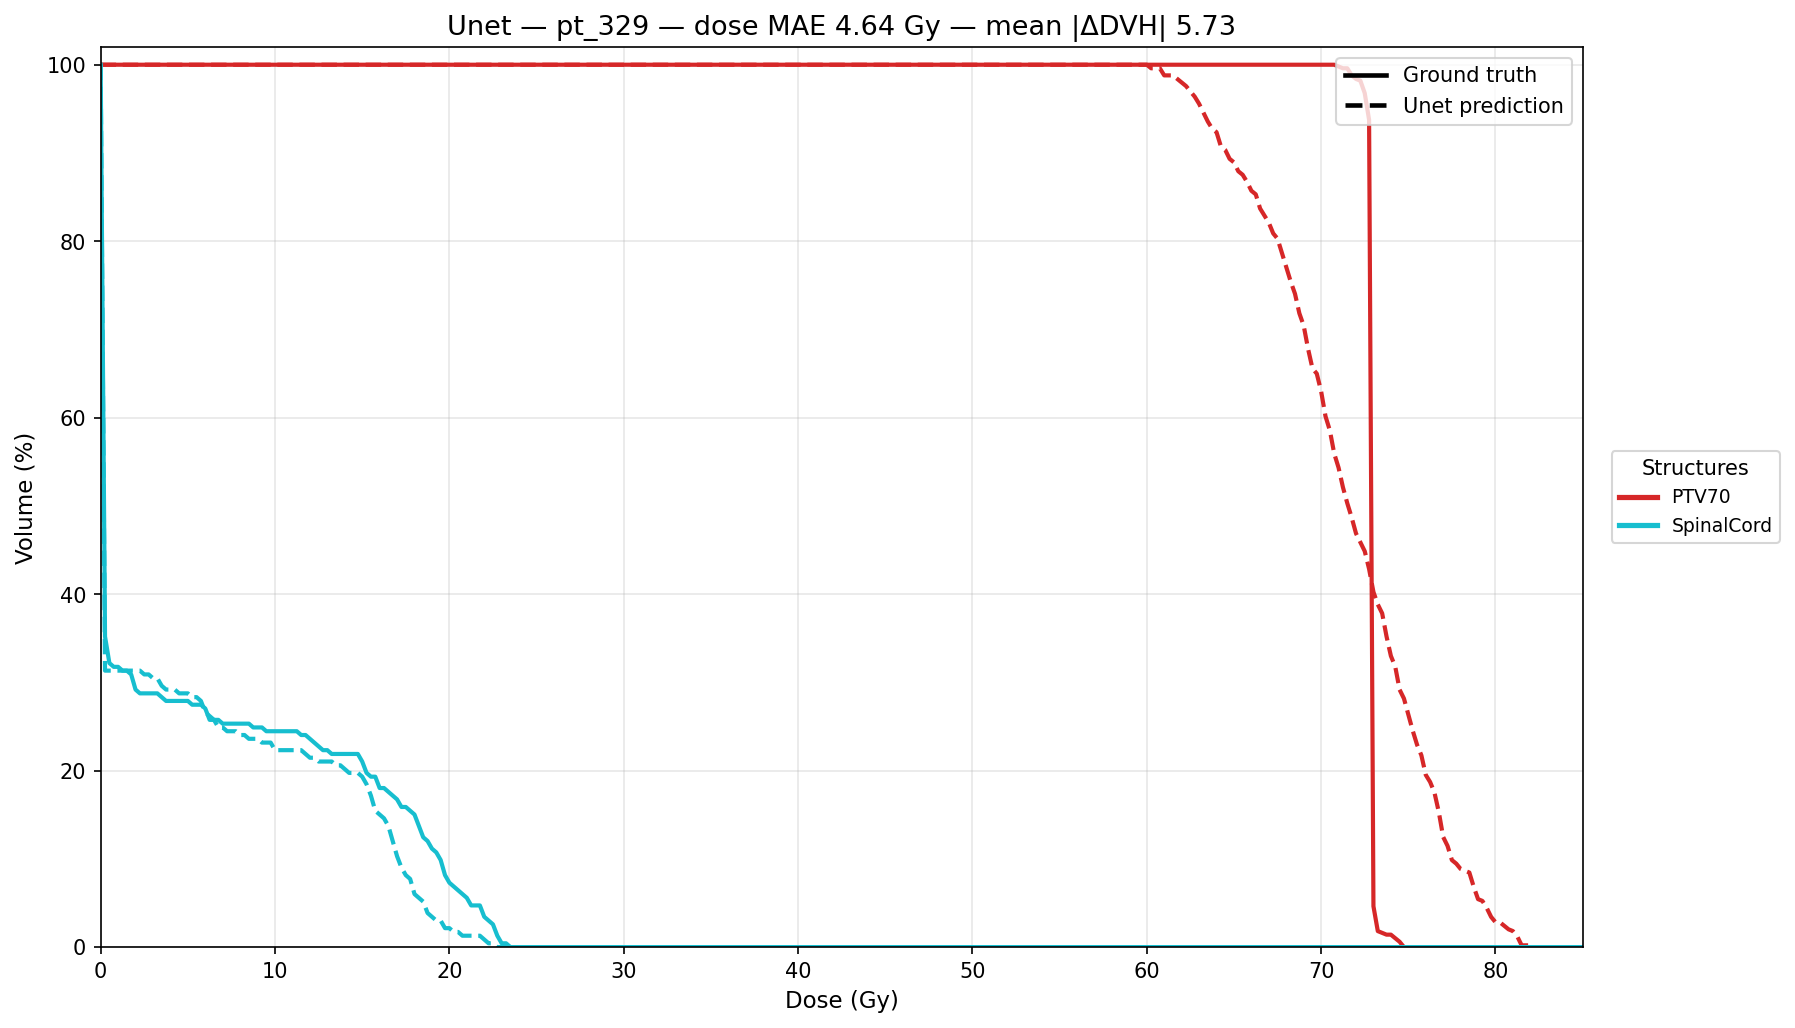
\includegraphics[width=0.493\textwidth]{Figures/pt329-unet.png}\hfill
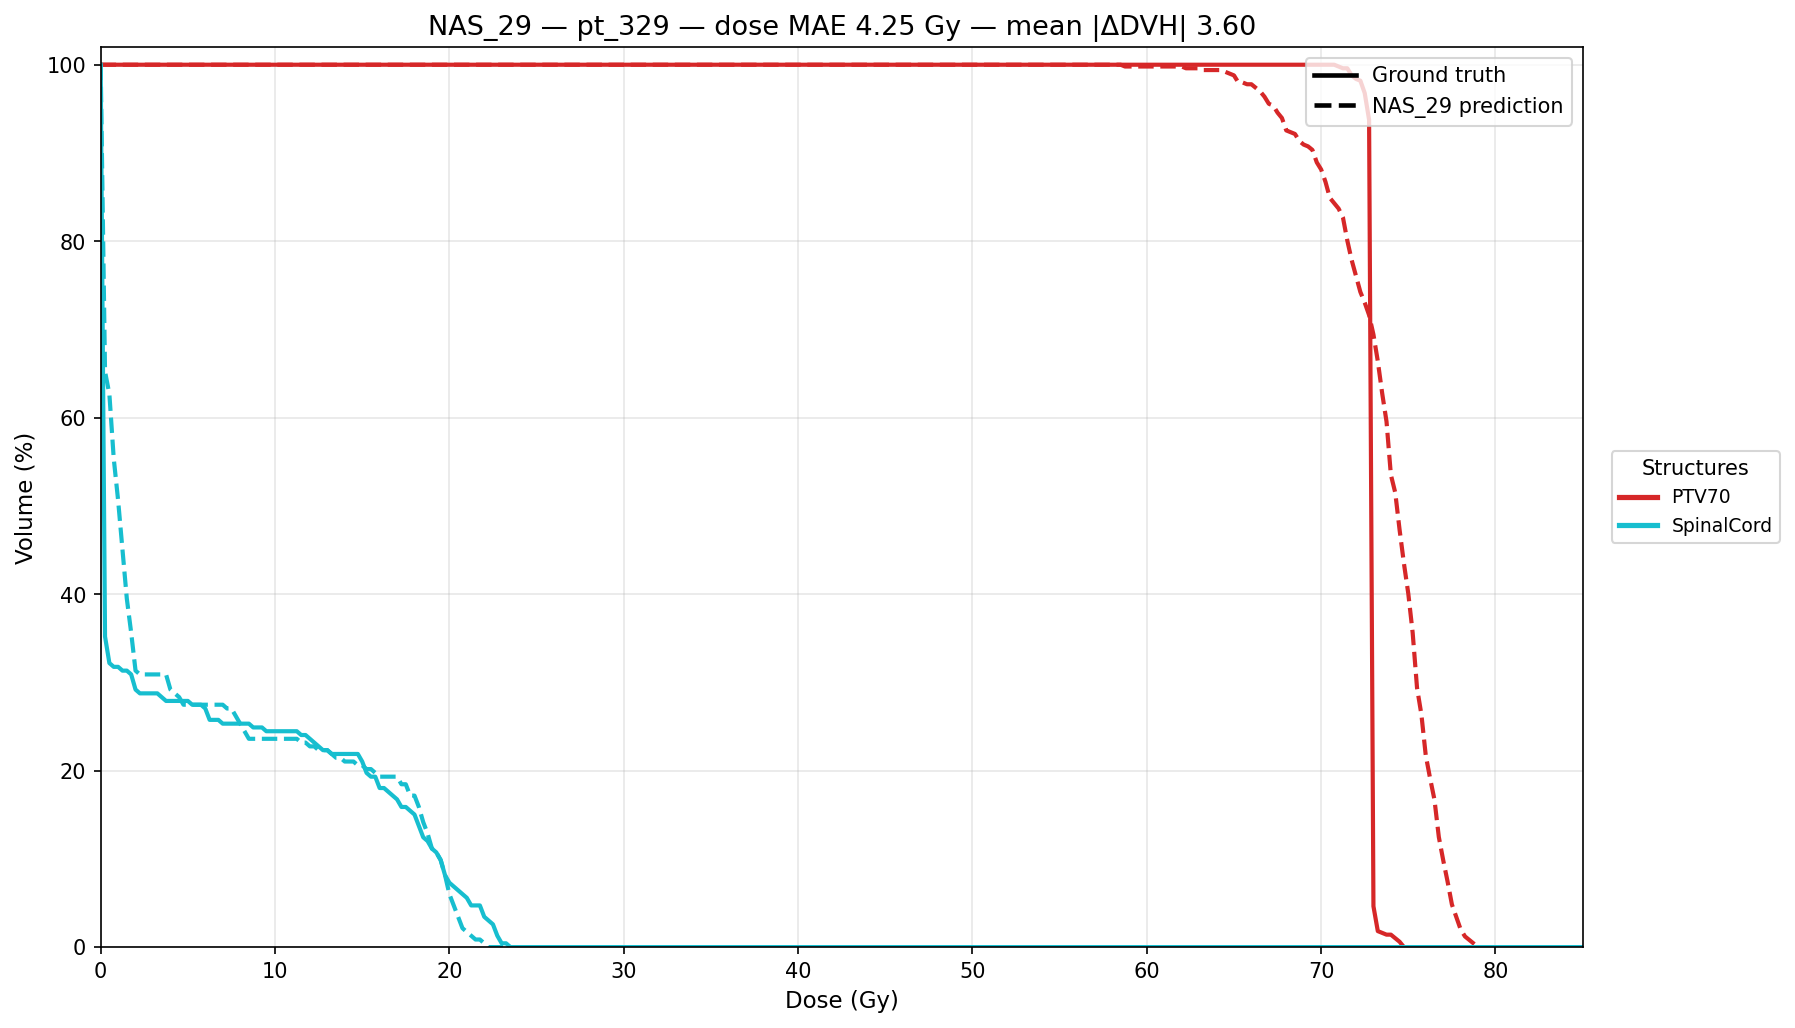
\includegraphics[width=0.493\textwidth]{Figures/pt329-nas29.png}
\caption{Cumulative DVHs for OpenKBP patient 329 with U-Net (left) and NAS-29 (right). Each plot overlays PTV70 (red) and spinal cord (cyan) on one set of axes. Solid curves show the reference and dashed curves show predictions. At 95\% target volume, NAS-29's predicted dose lies closer to the sharp reference falloff. We selected this case retrospectively for its large between-model difference.}
\label{fig:dvh}
\end{figure*}

\subsection{Endpoints and aggregation}
The dose score is the mean of $e_i$ over patients, giving each patient equal weight. For each available PTV we also compare $D_1$, $D_{95}$ and $D_{99}$, where $D_x$ is the dose received by at least $x$\% of the target. For each available OAR we compare mean dose and the near-maximum dose to its hottest 0.1 cubic centimeters, accounting for voxel spacing. Each comparison contributes an absolute error in Gy. The pooled DVH score gives equal weight to each available patient--structure--endpoint entry. Consequently, patients with more delineated organs receive more weight in this particular score.

For clarity, we also compute each patient's mean DVH endpoint error and describe the distribution of these 100 means. The pooled DVH standard deviation summarizes variation among 1,783 entries, whereas the patient-level standard deviation gives variation between individuals. All standard deviations below describe the observed population, using divisor $n$. The reported ranges are observed minima and maxima. We matched both models' records on patient, structure and endpoint before calculating differences.





\subsection{Patient- and Structure-Level Results}
Compared with U-Net, NAS-29 lowered mean dose error by 0.098 Gy (3.7\%) and pooled DVH error by 0.146 Gy (8.1\%) (Table~\ref{tab:results}). Dose error favored NAS-29 in 73 of 100 patients, and mean within-patient DVH error favored it in 60. We estimated uncertainty across patients by drawing 10,000 paired bootstrap samples of size 100 (seed 29). Each sampled patient contributed all available DVH entries to the recalculated pooled score. The 95\% percentile intervals for the error reductions were 0.050--0.146 Gy for dose and 0.064--0.230 Gy for DVH. Both intervals are conditional on the two trained checkpoints.

All 100 test patients had a PTV70 contour. Of its three endpoints, $D_{95}$ showed the largest reduction in mean absolute error, from 1.876 to 1.409 Gy (Table~\ref{tab:endpoints}). Mean dose estimates also improved for both parotid glands. Spinal cord near-maximum dose showed the opposite pattern: across 88 patients with a cord contour, mean absolute error increased by 0.329 Gy. Reporting endpoint-specific errors and denominators makes this tradeoff visible even when both aggregate scores favor the same model.

\begin{table}[t]
\centering
\begin{tabular}{lrrr}
\toprule
Structure and endpoint & $n$ & U-Net & NAS-29\\
\midrule
PTV70 $D_1$ & 100 & 1.868 & 1.744\\
PTV70 $D_{95}$ & 100 & 1.876 & 1.409\\
PTV70 $D_{99}$ & 100 & 2.141 & 1.863\\
Brainstem $D_{0.1\mathrm{cc}}$ & 89 & 2.712 & 2.418\\
Spinal cord $D_{0.1\mathrm{cc}}$ & 88 & 1.887 & 2.216\\
Left parotid mean & 98 & 1.665 & 1.450\\
Right parotid mean & 99 & 1.561 & 1.389\\
\bottomrule
\end{tabular}
\caption{Mean absolute error (Gy) for selected target and OAR endpoints. The same $n$ patients contribute to both models in each row.}
\label{tab:endpoints}
\end{table}



\subsection{Visualization Analysis}
Figure~\ref{fig:dvh} compares cumulative DVHs from the two predictors with the same reference curves. At a fixed volume fraction, their horizontal separation from the reference gives the absolute dose error. For visualization, we selected the patient with the largest reduction in mean DVH error among those whose two scores both favored NAS-29. Patient 329 had two delineated structures and five DVH endpoints. Dose error decreased from 4.643 to 4.253 Gy and mean DVH error from 5.729 to 3.599 Gy. Dose error remained above the respective cohort means for both models.

The largest visual difference occurs along the PTV70 falloff. At 95\% of target volume, the reference dose is 72.71 Gy. The U-Net curve crosses this level at 63.18 Gy and the NAS-29 curve at 67.46 Gy. At $D_{99}$, the absolute error likewise decreases from 10.75 to 6.95 Gy. Both models underestimate target coverage. For the hottest 0.1 cc of spinal cord, the reference dose is 22.77 Gy, compared with 21.99 Gy for U-Net and 21.42 Gy for NAS-29. Thus the reduction in overall DVH error in this example is driven primarily by better agreement over the target.

\section{Interpretation and Limitations}
Under the shared training protocol, one SearchedNet configuration achieved lower errors on both benchmark scores than the fixed U-Net. The comparison concerns the complete predictors. They differ in parameter count and in several operations, so the observed differences cannot be attributed to a particular encoder or upsampling operator. NAS-29 was specified before these runs. Evaluating the agent's contribution will require a separate comparison in which competing selection strategies have access to the same architecture space and computational budget.

The proposed comparison of training manifests also has limits. At a fixed number of optimizer updates, excluding cases increases the expected number of draws per remaining patient. Any change in performance could reflect that change in exposure as well as annotation quality or case mix. We would report both the update count and the exposure per patient. Reuse of validation data for screening architectures, selecting checkpoints and comparing manifests further limits the interpretation of the best validation score. External testing is particularly important because the present OpenKBP comparison informed the design of the proposed search.

\section{Future Work}
The first implementation study will assess whether a reviewer can reconstruct each selection decision from its recorded inputs and outputs. We plan to archive the controller version, prompts and decoding settings, tool versions, hardware measurements, seeds, manifests, effective optimizer groups and rejected trials. Reviewers will trace a claimed improvement to a matched comparison and identify explanations that remain unresolved because several operations changed together. For the Bridge working session, we propose using the event schema and the DVHs from patient 329 to elicit the records physicists and AI researchers need when they question a model choice.

We will compare the agent with fixed U-Net, fixed NAS-29 and a budget-matched search that samples the same operators and recipes without cohort measurements. Ablations will isolate data filtering, evidence-guided proposals and tuning. Repeated seeds will quantify selection stability, computational cost and how often matched trials support an exclusion. We will also evaluate the configurable nnDoseNet framework and the distance-aware diffusion model DoseDiff on common splits and endpoints \citep{nndose,dosediff}. If either improves target or organ dose estimates under comparable resources, we will test whether allowing the agent to choose among these model families further improves prediction.

External evaluation will include independent cohorts from other institutions and anatomical sites, including prostate radiotherapy. Before transfer, we will reconcile prescriptions, contour definitions and acquisition geometry, then lock each external test set before model selection. We will report error and coverage for small or infrequently delineated structures and invite clinical reviewers to examine cases in which voxelwise and DVH scores disagree. This evaluation will test both generalization to new patients and the ability to trace a deteriorating endpoint back to the evidence used in model selection.

\paragraph{AI assistance.} OpenAI Codex (GPT-6) assisted with manuscript drafting, literature discovery, tabulation of archived results and LaTeX preparation. The reported dose predictions come from the two trained neural networks. The proposed language-model controller has not been run in these experiments.

\bibliography{references}
\end{document}
